%%% Local Variables:
%%% mode: latex
%%% TeX-master: "../doc"
%%% coding: utf-8
%%% End:
% !TEX TS-program = pdflatexmk
% !TEX encoding = UTF-8 Unicode
% !TEX root = ../doc.tex
Das Resultat besteht wie beschrieben aus verschiedenen Artefakten. In diesem Abschnitt wird konkret auf die Resultate der verschiedenen Schritte eingegangen und der Zusammenhang hergestellt.

\section{LOD Pipeline}

Der Kern der Arbeit stellt die LOD-Pipeline, \e{lode} genannt, dar. Dieses Tool liefert eine für das Web optimierte Möglichkeit, LOD-Artefakte für eine Vielzahl von Anwendungsgebieten zu generieren.

\subsection{Aktueller Workflow}

Der übliche Ablauf für das Generieren von LOD-Artefakten ist wie folgt:
Für ein gegebenes Modell werden innerhalb vom Modellierungstool wie zum Beispiel Blender bestimmte LOD-Stufen von Hand generiert. Anschliessend werden die verschiedenen Stufen exportiert und manuell in die Applikation integriert. \e{Fine Tuning} erfordert sowohl Anpassungen an den Modellen als auch im Code. Erst muss im Modellierungstool die Anpassung manuell vorgenommen, dann neu in die Applikation geladen und dort neu geprüft werden. Diese Schritte können sich mehrfach wiederholen, was mühselig und teuer ist.

\todo[inline]{@marc Step by step anleitung? (von blender zu justierung in Three.js)}

\subsection{lode Pipeline}

Das Ziel von \e{lode} ist es, für ein möglichst breites Spektrum von Anwendungsfällen eine einfache Lösung anzubieten und somit die Hemmschwelle für den Einsatz von LOD-Artfakten zu reduzieren.

Deshalb setzt \e{lode} konsequent auf moderne Entwicklungsprozesse, die nahtlos in die bestehenden Prozesse integriert werden können. Manuelle Schritte sollen auf ein Minimum reduziert und Finetuning so einfach wie möglich werden.

\subsection{lode Ablauf}

Der Ablauf der \e{lode}-Pipeline kann in drei Schritte unterteilt werden.

\paragraph{Setup und Konfiguration}
3D-Modelle werden erstellt und als glTF-Dateien innerhalb des Projekts gespeichert. Eine zu den Modellen gehörige Konfigurationsdatei (Abbildung \ref{fig:lodeConfigFile}) kann mittels \e{CLI}, welches auf \e{NPM} verfügbar ist, angelegt werden (wie in Abbildung \ref{fig:lodecliconfig} dargestellt).

\begin{figure}[H]
  \begin{lstlisting}
    {
      "levels": [
        {
          "threshold": 300
        },
        {
          "threshold": -1,
          "configuration": {
            "targetScale": 0.0625
          }
        }
      ]
    }
  \end{lstlisting}
\caption{Durch das CLI generierte Konfigurationsdatei}
\label{fig:lodeConfigFile}
\end{figure}

\begin{figure}[H]
  \centering
  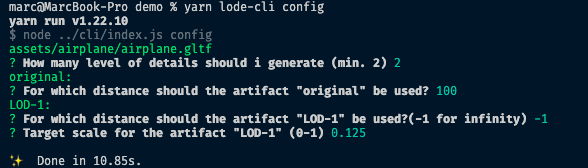
\includegraphics[width=0.8\columnwidth]{resultate/screenshotlodecliconfig.png}
  \caption{lode \e{CLI} config – Konfiguriert die gewünschten LOD-Artefakten}
  \label{fig:lodecliconfig}
\end{figure}

\paragraph{Erstellen der Artefakte}
Danach generiert \e{lode} die in der Konfigurationsdatei beschriebenen LOD-Artefakte (in Abbildung \ref{fig:lodeclirun} ersichtlich). Wenn sich ein Modell oder eine Konfiguration ändert, werden die notwendigen Schritte automatisch erneut durchgeführt. So ist es möglich, schnell Anpassungen vorzunehmen und die Änderungen im Projekt ohne manuelle Arbeit zu sehen.

\begin{figure}[H]
  \centering
  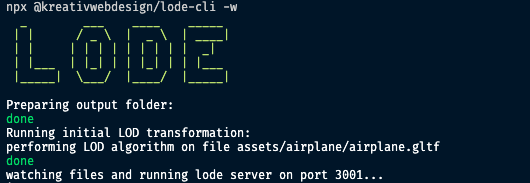
\includegraphics[width=0.8\columnwidth]{resultate/screenshotlodeclirun.png}
  \caption{lode \e{CLI} run – Generiert die gewünschten LOD-Artefakten}
  \label{fig:lodeclirun}
\end{figure}

Das zugehörige \e{lode-ui} (in Abbildung \ref{fig:lodeui} gezeigt) bietet zudem die Möglichkeit, die verschiedenen Detailstufen miteinander zu vergleichen und die Konfiguration möglichst einfach zu justieren. Dies ermöglicht es, die Änderungen in Echtzeit zu sehen und die Distanzen, bei welchen Level aktiviert werden, einzustellen. So ist kein manuelles hin und her wechseln zwischen Applikationen mehr notwendig.

\begin{figure}[H]
  \centering
  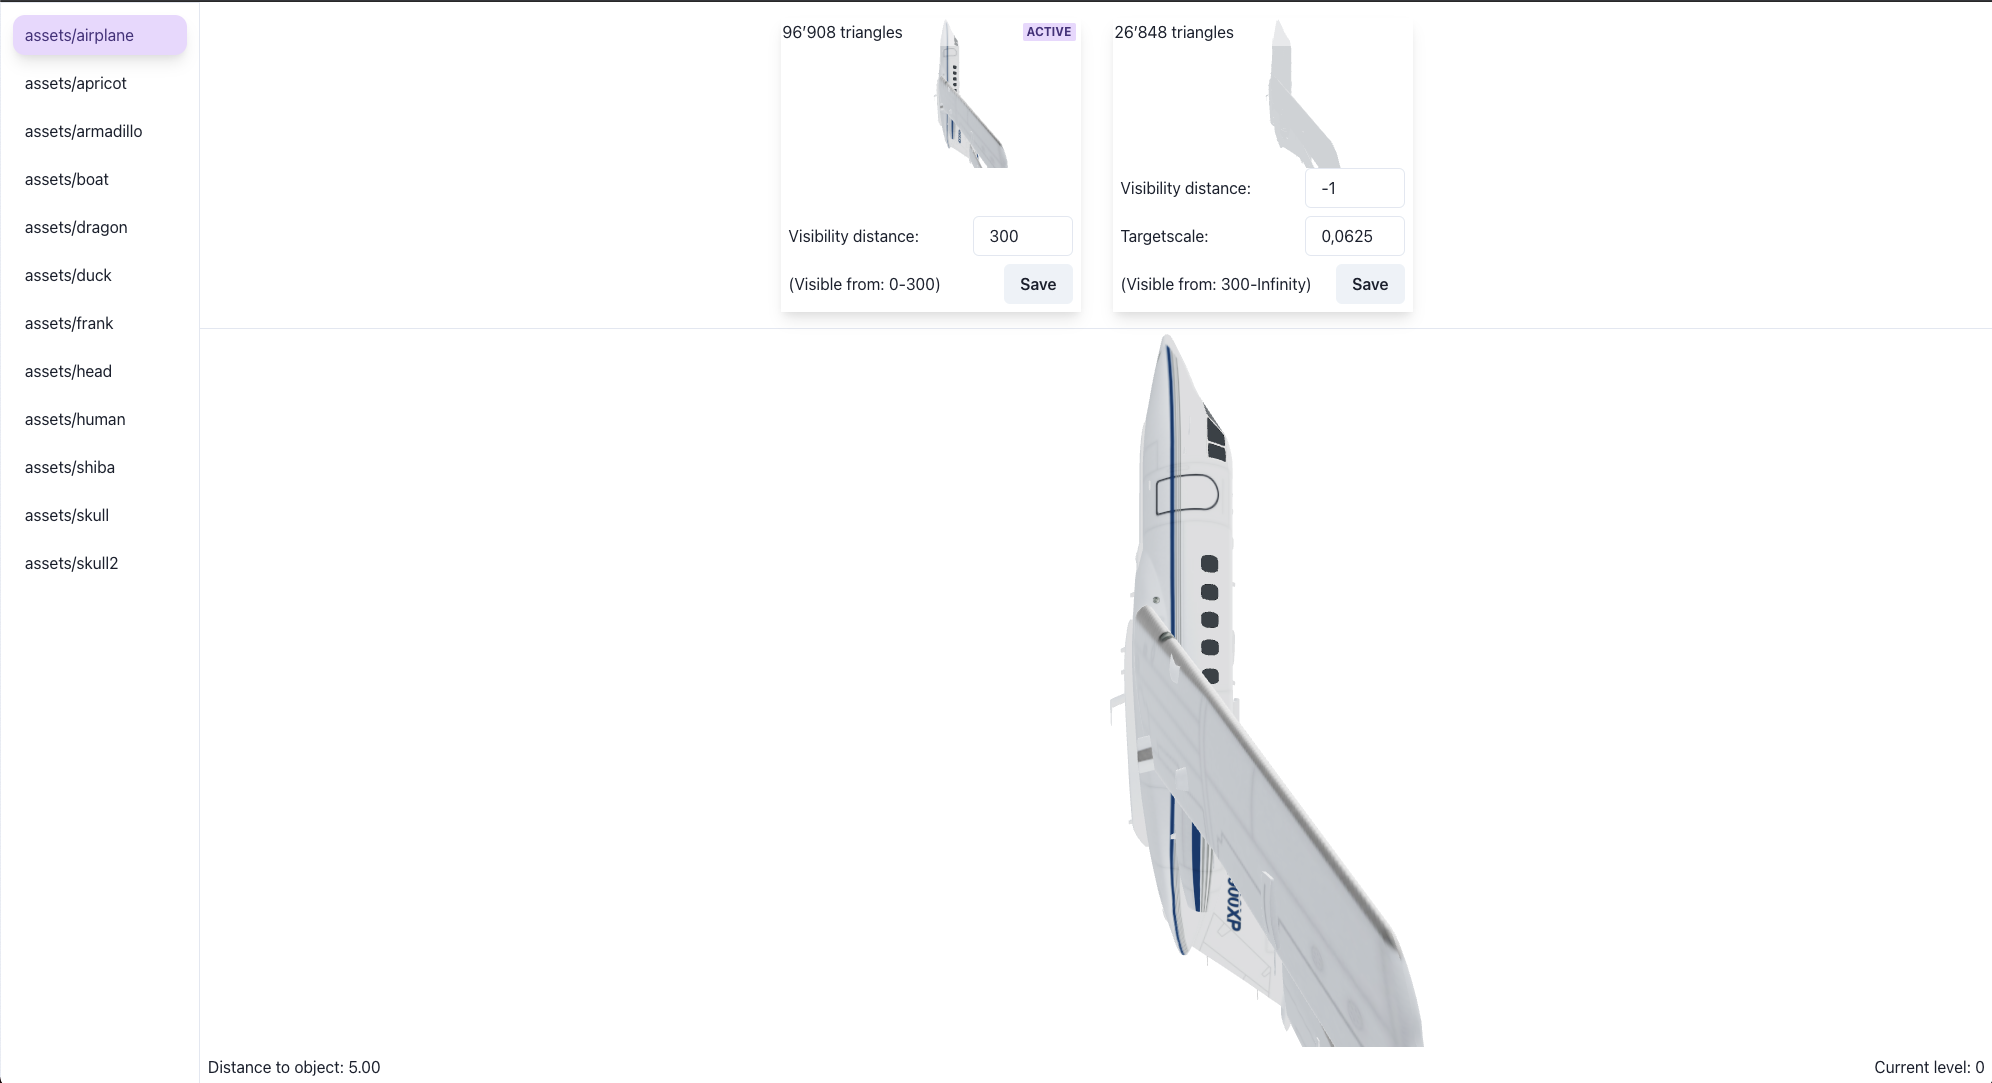
\includegraphics[width=1\columnwidth]{resultate/screenshotlodeui.png}
  \caption{lode-ui}
  \label{fig:lodeui}
\end{figure}

\paragraph{Verwendung der Artefakte in der Applikation}
Die Artefakte können innerhalb der Applikation mithilfe einer Bibliothek geladen werden. Dabei werden die Definitionen in der Konfigurationsdatei geladen und das Modell entsprechend in der Szenerie dargestellt, wie in Beispielcode \ref{code:lodeThreeUsage} zu sehen ist.

\begin{figure}[H]
  \begin{lstlisting}[style=JavaScript]
  import * as lodeLoader from "lode-three";
  import manifest from "./lode-build/lode-manifest.json";

  const lodeContext = lodeLoader.createContext({
    manifest,
    basePath: "./lode-build",
  });

  const airplaneModel = await lodeLoader.loadModel({
    lodeContext,
    artifactName: 'assets/airplane',
  })

  scene.add(airplaneModel)
  clone.position.set(0, 0, 0);
  \end{lstlisting}
  \caption{Beispielcode zur Benutzung der LOD-Artefakte mittels \e{lode-three} in \e{Three.js}}
  \label{code:lodeThreeUsage}
\end{figure}

\section{LOD Generierung}

Für das Erstellen von LOD-Artefakten wurde ein für LOD-Artefakte optimierte Version des in \autoref{chap:surfaceSimplificationAlgorithm} erklärten \e{Surface Simplification Algorithmus} entwickelt.

\subsection{Implementation}

Die Implementation des Algorithmus wurde in JavaScript, basierend auf \fGls{Node.js}{JavaScript Ausführungsumgebung, welche ohne einen Browser verwendet werden kann}, umgesetzt. Grund dafür ist das Einbinden von \e{lode} in bestehende Entwicklungsabläufe in der Webentwicklung. So ist es einfach möglich, das Paket kostenlos mithilfe von \gls{npm} zur Verfügung zu stellen.

\todo[inline]{@simon mehr details über Implementation: boundary normalization, optimal point, matrices, detailablauf...}

\subsection{Artefakte}

Die generierten Artefakte sind unabhängig voneinander. So ist es nicht notwendig alle Artefakte zu jeder Zeit zu laden. Dies hat den primären Vorteil, dass es möglich ist, progressives Laden als Erweiterung zuzulassen. Progressives laden bedeutet, dass zuerst die LOD-Artefakte mit den wenigsten Details geladen werden und angezeigt werden bis die detaillierteren Level visualisiert werden.
Es ist sogar möglich, auf gewissen Geräten die detaillierten Level überhaupt nicht zu laden und so zum Beispiel Bandbreite zu sparen.

\subsection{Fehlermetrik}

Die Fehlermetrik wurde vergleichbar mit der Referenzimplementation justiert. Die Referenzimplementation setzt auf absolute Fehlerwerte. Dies hat zur Konsequenz, dass abhängig von der Skalierung des Modells potenziell zu viel oder zu wenige \e{Edge Collapses} durchgeführt werden. Ein Modell mit geringer Skalierung generiert tiefere Werte für die Fehlermetrik und umgekehrt. Um diesem Umstand gerecht zu werden, wird vorab die Skalierung der Modelle normalisiert. Die \e{Vertices} werden dabei um einen modellabhängigen Faktor angepasst. So haben alle Modelle eine vergleichbare Basis für die Fehlermetrik und starke Unterschiede zwischen verschiedenen Modellen können vermieden werden.

\subsection{Texturen}

Bei vielen Modellen sind der grösste Teil der Speichergrösse die Texturen. Das Optimieren der geometrischen Struktur reduziert die zugehörigen Texturen jedoch nicht. Um trotzdem möglichst grosse Einsparungen für die Texturen zu ermöglichen wurde eine Methode entwickelt, welche versucht die prominenteste Farbe eines Modells zu extrahieren und diese für die Vereinfachungen zu verwenden.
In Abbildung \ref{fig:textureComparison} ist dieser Unterschied visualisiert.
Diese Technik führt zu signifikanten Detailverlusten bei der Nahbetrachtung und ist somit ungeeignet für das Verwenden bei der ersten LOD-Stufe. Für alle weiteren Stufen überwiegt jedoch der Vorteil der Vereinfachung im Vergleich zum Detailverlust.
\begin{figure}[H]
  \centering
  \begin{subfigure}{.4\textwidth}
    \centering
    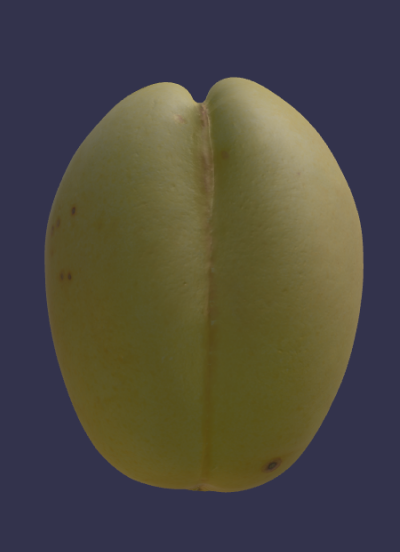
\includegraphics[width=.8\linewidth]{resultate/lod-original-texture.png}
    \caption{Original Textur}
  \end{subfigure}
  \begin{subfigure}{.4\textwidth}
    \centering
    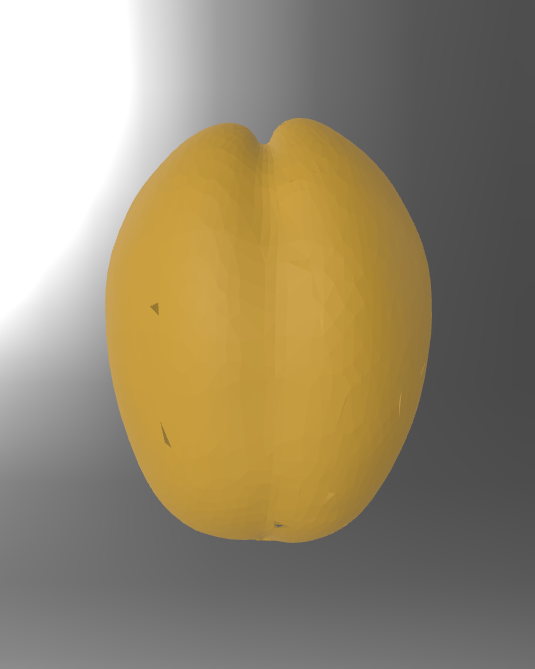
\includegraphics[width=.8\linewidth]{resultate/lod-simplified-texture.png}
    \caption{Vereinfachte Textur}
  \end{subfigure}
  \caption{Vergleich der Texturen}
  \label{fig:textureComparison}
\end{figure}

\todo[inline]{@marc screenshots im studio modus}

\subsection{Vergleich}

Unter Berücksichtigung der Auswirkungen auf die Downloadgrösse wird der Einsatz von zwei Stufen empfohlen: das Original und das Vereinfachte.

In Abbildung \ref{fig:lodComparison} ist eine solche Vereinfachung neben dem zugehörigen Original ersichtlich. Beim Original handelt es sich um ein Modell mit 4212 \e{Triangles}. Die Vereinfachung hat lediglich noch deren 269. Während das Original eine Dateigrösse von 122 KB aufweist, hat die Vereinfachung lediglich 6 KB. Vergleichbare Relationen treten auch mit komplexeren Modellen auf.

\begin{figure}[H]
  \centering
  \begin{subfigure}{.4\textwidth}
    \centering
    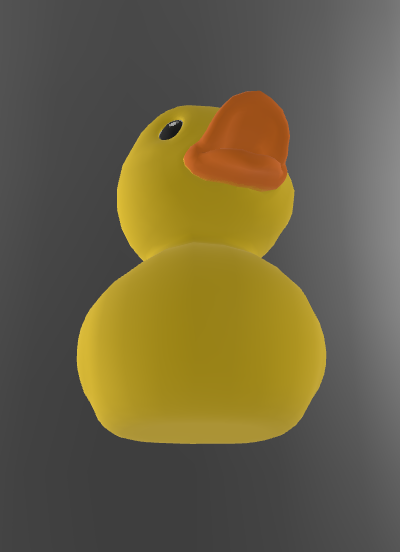
\includegraphics[width=.8\linewidth]{resultate/lod-original.png}
    \caption{Originalmodell}
  \end{subfigure}
  \begin{subfigure}{.4\textwidth}
    \centering
    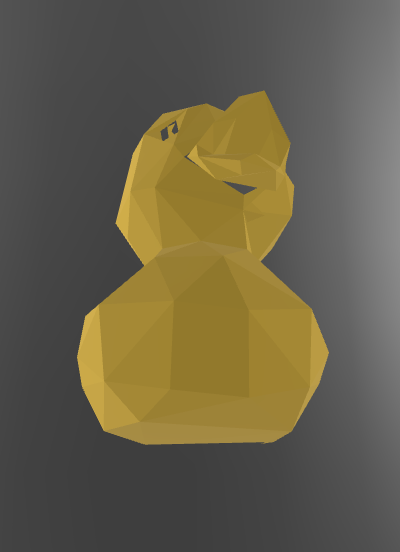
\includegraphics[width=.8\linewidth]{resultate/lod-simplified.png}
    \caption{vereinfachtes Modell}
  \end{subfigure}
  \caption{Vergleich Originalmodell und vereinfachtes Modell}
  \label{fig:lodComparison}
\end{figure}

Bei einer Nahbetrachtung der Modelle sind die Unterschiede klar ersichtlich. Bei einer gewissen Distanz sind die Differenzen der beiden Modelle unauffälliger. In Abbildung \ref{fig:lodComparisonDistance} werden dieselben Modelle auf eine Distanz von 72 (m) dargestellt. Die Standardeinstellung für die maximale Distanz des Kamera Frustum liegt bei Babylon.js zum Beispiel bei 10'000 (m) \cite{babylonMaxZ}. Auf diese Distanz kann der orange Schnabel beim Originalmodell noch knapp erkannt werden - andere Details sind auf diese Distanz jedoch nicht ersichtlich.

\begin{figure}[H]
  \centering
  \begin{subfigure}{.4\textwidth}
    \centering
    
\includegraphics[width=.8\linewidth]{resultate/original-distance.png}
    \caption{Originalmodell}
  \end{subfigure}
  \begin{subfigure}{.4\textwidth}
    \centering
    
\includegraphics[width=.8\linewidth]{resultate/simplified-distance.png}
    \caption{vereinfachtes Modell}
  \end{subfigure}
  \caption{Vergleich Originalmodell und vereinfachtes Modell auf Distanz}
  \label{fig:lodComparisonDistance}
\end{figure}

\section{Benchmark}

Das Ziel des Benchmarks ist der Vergleich einer Version ohne Einsatz von LOD und einer Umgebung, welche LODs einsetzt. Um eine möglichst praxisnahe Aussage treffen zu können, wird hierfür eine Demo-Szenerie verwendet, welche einer echten Anwendung so nah wie möglich kommt. Somit wird gewährleistet, dass es nicht nur in der Theorie einen Nutzen für LODs gibt, sondern dieser in der Praxis vorhanden ist.

\paragraph{Browser Umgebung}
Um den Umfang des Benchmarks überschaubar zu halten, wurde ausschliesslich ein Benchmark für Google Chrome entwickelt.
Google Chrome basiert auf \fgls{Chromium}{Open Source Browser-Projekt, welches von Google entwickelt wird. Andere Browser basieren ebenfalls auf der Code-Basis von Chromium. Namentlich Microsoft Edge und Opera, um die bekanntesten zu nennen}, dieselbe Engine, welche auch Microsoft Edge oder Opera verwenden.
Einen Benchmark basierend auf Google Chrome liefert somit auch Indizien für diese beiden Browser, auch wenn gewisse Abweichungen möglich sind.
Neben dem Marktführer Chrome sind Mozilla Firefox oder Safari von Apple ebenfalls Optionen. Jedoch wurde primär aufgrund des Marktanteils von total rund 70\% \cite{browserUsage} zugunsten von Google Chrome entschieden.
Die getroffenen Aussagen bezüglich Laufzeitverhalten behalten ihre Gültigkeit auch für andere Browser.

\paragraph{Automation}
Um die Tests durchzuführen, wird ein Testautomationstool benötigt; unter anderem der Einsatz von Selenium wurde in Erwägung gezogen.
Der Vorteil von Selenium ist insbesondere, dass der Benchmark für weitere Browser ausgeweitet werden könnte.
Da jedoch das Analysieren der GPU Daten stark vom System abhängig ist und dafür zusätzliche Komplexität notwendig wäre, wird in diesem Benchmark die im Google Chrome integrierten \e{Chrome DevTools} eingesetzt.
Selenium bietet zurzeit eine suboptimale Integration für das \e{Chrome DevTools Protocol}.
Um mögliche Diskrepanzen zwischen Systemen möglichst gering zu halten, wurde jedoch entschieden, auf die bewährte Lösung von Google Chrome zu setzen.
\fgls{Puppeteer}{Node.js Library, die eine API anbietet zum Steuern von \gls{Chromium} oder Chrome über das Chrome DevTools Protocol}, eine weitere Option für die Automation, ist eine Bibliothek, die eine vereinfachte Schnittstelle zu einer Chromium Instanz bietet.
Sie wird zudem direkt von Google entwickelt und bietet somit eine stabile Grundlage zur Kommunikation mit den \e{Chrome DevTools}.

\paragraph{Profiling}
Die \e{Chrome DevTools} erlauben es, ein detailliertes Laufzeitprofil einer Applikation anzulegen.
Im Profil befinden sich Informationen zu CPU- und GPU-Auslastung, aber auch generelle Informationen bzgl. der \gls{Rendering Engine} werden gesammelt.
Die Analyse dieser Daten ermöglicht es, eine Aussage zum Laufzeitverhalten einer Applikation zu tätigen.

\paragraph{Testaufbau}
Derselbe Testablauf wird sowohl für die optimierte als auch für die unoptimierte Version verwendet.
Bei einem Testablauf werden folgende Schritte durchlaufen:

\begin{enumerate}
  \item Öffne die Applikation in einer \emph{Chromium} Instanz.
  \item Warte bis die Seite geladen ist.
  \item Starte das \emph{Profiling}.
  \item Warte $n$ Sekunden.
  \item Stoppe das \emph{Profiling}.
  \item Werte die Daten aus.
\end{enumerate}

Der Test erfasst die in Tabelle \ref{table:benchmarkFigures} aufgeführten Kennzahlen.

\begin{table}[H]
  \centering
  \begin{tabular}{ l p{8cm} }
  \hline
  Kennzahl & Beschreibung \\
  \hline
  \hline
  Median \e{\gls{FPS}} & Die \e{\gls{FPS}} werden kontinuierlich berechnet. Um starke Abweichungen zu verwerfen wird der Median verwendet. \\
  \hline
  Dauer für das Laden der Modelle & Totale Zeit für das Laden aller Modelle der Szenerie. Dieser Wert ist relativ zu betrachten, da die Modelle lokal geladen werden und die Zeit für das Laden von einem Server signifikant höher sein kann. Grundsätzlich besteht eine ausreichende Korrelation zwischen Dateigrösse und Zeit für das Laden der Modelle. Ein zusätzlicher Faktor ist jedoch die Anzahl an Dateien, welche geladen werden müssen. \\
  \hline
  Median \e{Render Loop} Dauer & Der Median aller Laufzeiten der \e{Render Loop}. \\
  \hline
  Anzahl \e{Render Loop} Iterationen & Wie oft wurde ein neues Bild gezeichnet. Umso höher die Zahl, desto mehr verschiedene Frames konnten gerendert werden. \\
  \hline
  Totale GPU Zeit & Die totale Zeit, welche die GPU für Berechungen benötigt. \\
  \hline
  Anzahl GPU Events & Anzahl der Events an die GPU. Dieser Wert soll lediglich dazu dienen um die gemessenen \e{FPS} und die Anzahl \e{Render Loop} Iterationen besser einschätzen zu können. Eine höhere Anzahl an GPU Events steht innerhalb der Demoszenerie im Zusammenhang mit mehr \e{Render Loop} Iterationen. \\
  \hline
  \end{tabular}
  \caption{Kennzahlen für Benchmark}
  \label{table:benchmarkFigures}
\end{table}

\paragraph{Aufbau Testapplikation}
\label{chap:testApplication}
Die Testapplikation stellt eine komplexe Szenerie dar. Der Betrachter fliegt während dem Ablauf kontinuierlich über die Szenerie. Dies stellt die optimalen Bedingungen für den Einsatz von LOD-Artefakten dar. Abhängig von einem URL-Parameter wird entschieden ob LOD-Artefakte verwendet werden sollen oder nicht. Die Anwendung wurde mit Three.js implementiert. Bei der unoptimierten Version wird direkt das Originalmodell verwendet. Bei der optimierten Version werden mithilfe der LOD-Hilfsklasse die verschiedenen Artefakte geladen \cite{threeLODClass}.

In Abbildung \ref{fig:demoApplication} ist ein Screenshot der Testapplikation ersichtlich. Als Basis für die Applikation wurde Three.js eingesetzt. Die Kamera wird kontinuierlich innerhalb der Szene bewegt, die Position wird abhängig von der Systemzeit definiert. So ist es möglich, dass beide Applikationen – unabhängig von den \e{FPS} – jeweils die gleichen Aspekte innerhalb der Applikation visualisieren. Die Modelle werden zudem bei jedem Durchlauf identisch positioniert. Dies gewährleistet, dass das Laufzeitverhalten verlässlich ist.

Jedes Modell wird dabei mehrfach angezeigt, die Modelle werden einmal geladen und anschliessend mittels der \e{clone} Methode von Three.js geklont \cite{threeObject3DClone}. Dies stellt sicher, dass die Datenstruktur der Modelle nicht mehrfach in den Arbeitsspeicher geladen werden muss. Wichtig ist zu erwähnen, dass die Modelle bei dieser Methode mit mehreren \e{Draw Calls} gerendert werden. Der Einsatz von \e{InstancedMesh} wurde in Erwägung gezogen, zeigte jedoch keine nennenswerte Unterschiede zwischen der optimierten und unoptimierten Version \cite{threeInstancedMesh}.

\begin{figure}[H]
  \centering
  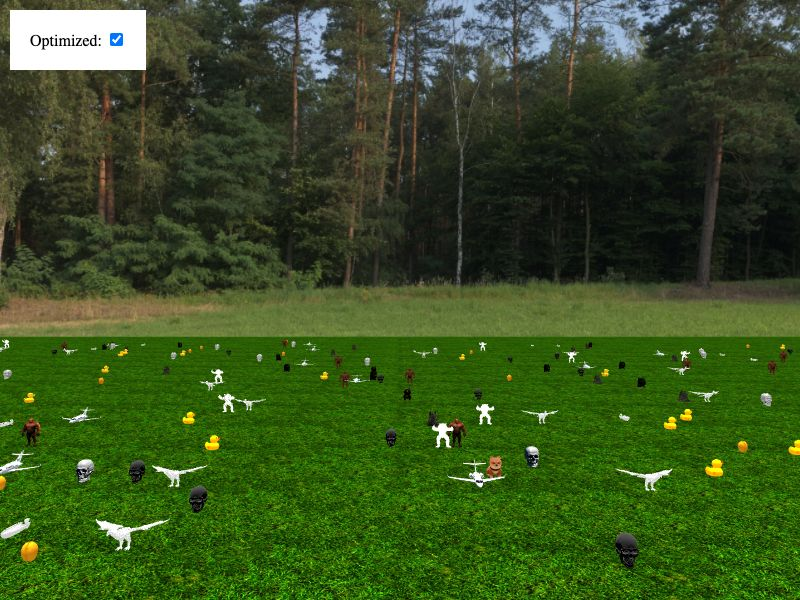
\includegraphics[width=0.8\columnwidth]{resultate/screenshotdemoapplication.jpg}
  \caption{Testapplikation}
  \label{fig:demoApplication}
\end{figure}

\paragraph{Testumgebung}
Um während den Tests möglichst faire Bedingungen zu gewährleisten, wird die Maschine zuvor wie bei anderen Benchmarks vorbereitet. Ziel ist es, Seiteneffekte zu minimieren. Für diesen Benchmark wurden deshalb die Instruktionen von \e{Tracer Bench} zur Behebung von Rauschen befolgt \cite{tracerBenchNoiseMitigation}. Die beiden Versionen werden jeweils abwechslungsweise ausgeführt, so wird sichergestellt, dass keine der beiden Varianten einen starken Nachteil durch Nebeneffekte erleidet. Ausserdem werden mehrere Durchläufe direkt nacheinander ausgeführt. Starke Abweichungen zwischen den Durchläufen würden bei der Analyse der Daten auffallen.

\paragraph{Analyse der Daten}
Für jeden Durchlauf wird der Median der \e{\gls{FPS}} Daten berechnet.
Anschliessend wird die Standardabweichung der \e{\gls{FPS}} für die unoptimierten respektive optimierten Werte berechnet. Die Standardabweichung dient als Kennzahl, um eine Signifikanz der Daten nachweisen zu können.

Zudem werden die weiteren erfassten Kennzahlen ausgewertet, um das Resultat der \e{\gls{FPS}} verifizieren zu können.

\subparagraph{Konfidenzintervall}
Die Signifikanz wird mithilfe eines statistischen Konfidenzintervalls nachgewiesen. Hierfür wird der Durchschnitt aller Mediane verwendet, zusätzlich wird ein Konfidenzintervall von 95\% gewählt. Es wird gewährleistet, dass das Resultat des Benchmarks verlässlich ist und für einen Vergleich verwendet werden kann. Überschneiden sich die Intervalle für die optimierte und unoptimierte Version kann keine statistische Signifikanz nachgewiesen werden. Grundsätzlich gilt: umso kleiner die Intervalle desto besser. Zudem sollten die beiden Intervalle möglichst weit entfernt voneinander liegen.

\subsection{Auswertung}
\label{chap:benchmarkResults}

Der Benchmark wurde auf verschiedenen Geräten ausgeführt. Im folgenden sind zwei Durchläufe mit jeweils 10 Proben erfasst.

Der erste Durchlauf wurde auf einem MacBook Pro durchgeführt. Wie in Abbildung \ref{fig:benchmarkFpsChartMarcbook} zu sehen, konnten die FPS auf 60 FPS gehoben werden im Vergleich zu den 48.2 FPS in der unoptimierten Version.
Direkt damit verbunden ist die Anzahl \e{Render Loop} Iterationen, welche genauso um ca 30\% gesteigert werden konnte. Auf der Umkehrseite wurde die Dauer für das Laden der Modelle etwas erhöht, da mehr Modelle geladen werden müssen (siehe \ref{fig:benchmarkDownloadChartMarcbook}). Diese wuchs aber nur um rund 10\%.

Die detaillierten Informationen befinden sich in Anhang \ref{fig:marcbookBenchmarkRun}.

\begin{figure}[H]
  \centering
  \begin{subfigure}{.49\textwidth}
    \centering
    \includegraphics[width=0.9\linewidth]{resultate/marcbook/fpsChart.jpg}
    \caption{FPS Vergleich}
    \label{fig:benchmarkFpsChartMarcbook}
  \end{subfigure}
  \begin{subfigure}{.49\textwidth}
    \centering
    \includegraphics[width=0.9\linewidth]{resultate/marcbook/downloadChart.jpg}
    \caption{Download Vergleich}
    \label{fig:benchmarkDownloadChartMarcbook}
  \end{subfigure}
  \caption{Vergleich Kennzahlen}
  \label{fig:benchmarkChartMarcbook}
\end{figure}

Auch der zweite Durchlauf auf einem Dell Gerät führt zu ähnlichen Daten. Auffallend in \ref{fig:benchmarkFpsChartWindows} ist der Unterschied der \e{FPS}. Hierfür muss bemerkt werden, dass es sich um eine integrierte Grafikkarte handelt. Die Unterschiede der Downloadzeit (siehe \ref{fig:benchmarkDownloadChartWindows}) sind vergleichbar mit denjenigen vom ersten Durchlauf.

Die detaillierten Informationen befinden sich in Anhang \ref{fig:windowsBenchmarkRun}.

\begin{figure}[H]
  \centering
  \begin{subfigure}{.49\textwidth}
    \centering
    \includegraphics[width=0.9\linewidth]{resultate/windows/fpsChart.jpg}
    \caption{FPS Vergleich}
    \label{fig:benchmarkFpsChartWindows}
  \end{subfigure}
  \begin{subfigure}{.49\textwidth}
    \centering
    \includegraphics[width=0.9\linewidth]{resultate/windows/downloadChart.jpg}
    \caption{Download Vergleich}
    \label{fig:benchmarkDownloadChartWindows}
  \end{subfigure}
  \caption{Vergleich Kennzahlen}
  \label{fig:benchmarkChartWindows}
\end{figure}
